

\tikzset{every picture/.style={line width=0.75pt}} %set default line width to 0.75pt        

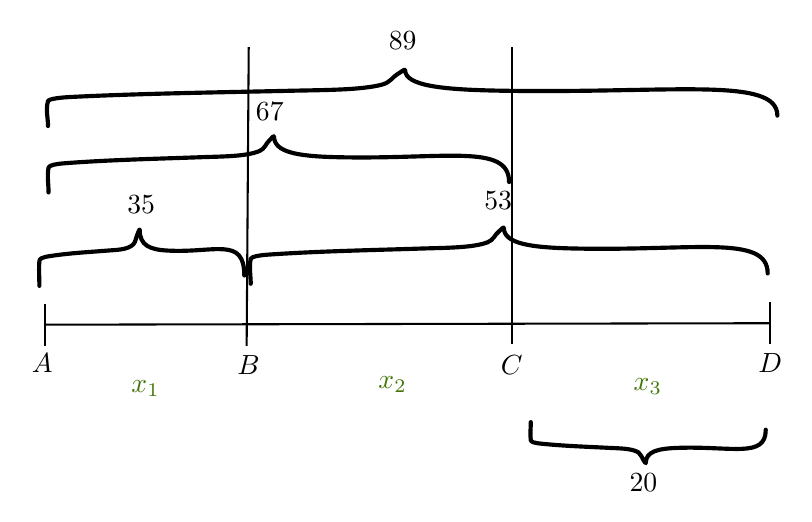
\begin{tikzpicture}[x=0.75pt,y=0.75pt,yscale=-1,xscale=1]
%uncomment if require: \path (0,300); %set diagram left start at 0, and has height of 300

%Straight Lines [id:da18809251009182648] 
\draw    (100,143) -- (449,142.29) ;
%Straight Lines [id:da4295294079118699] 
\draw    (100,132.85) -- (100,153.15) ;
%Straight Lines [id:da08559662247482214] 
\draw    (198,9.29) -- (197,153.15) ;
%Straight Lines [id:da8061715298122138] 
\draw    (325,9.29) -- (325,152.15) ;
%Straight Lines [id:da1891846903803609] 
\draw    (449,132.15) -- (449,152.44) ;
%Shape: Free Drawing [id:dp5156036617765727] 
\draw  [color={rgb, 255:red, 0; green, 0; blue, 0 }  ][line width=1.5] [line join = round][line cap = round] (101.3,47.29) .. controls (101.3,43.29) and (100.09,39.28) .. (101.3,35.29) .. controls (101.67,34.1) and (107.95,33.51) .. (112.28,33.29) .. controls (146.53,31.59) and (183.69,31.09) .. (218.43,30.29) .. controls (233.89,29.94) and (252.54,29.98) .. (262.36,27.29) .. controls (266.42,26.18) and (267.24,23.63) .. (269.68,22.29) .. controls (270.9,21.63) and (273.34,19.55) .. (273.34,20.29) .. controls (273.34,27.91) and (291.11,29.83) .. (320.92,30.29) .. controls (402.67,31.57) and (452.7,23.35) .. (452.7,42.29) ;
%Shape: Free Drawing [id:dp895862543035038] 
\draw  [color={rgb, 255:red, 0; green, 0; blue, 0 }  ][line width=1.5] [line join = round][line cap = round] (101.56,79.29) .. controls (101.56,75.29) and (100.79,71.28) .. (101.56,67.29) .. controls (101.79,66.1) and (105.76,65.51) .. (108.49,65.29) .. controls (130.11,63.59) and (153.58,63.09) .. (175.52,62.29) .. controls (185.28,61.94) and (197.06,61.98) .. (203.25,59.29) .. controls (205.82,58.18) and (206.34,55.63) .. (207.88,54.29) .. controls (208.65,53.63) and (210.19,51.55) .. (210.19,52.29) .. controls (210.19,59.91) and (221.41,61.83) .. (240.24,62.29) .. controls (291.85,63.57) and (323.44,55.35) .. (323.44,74.29) ;
%Shape: Free Drawing [id:dp019817472694717342] 
\draw  [color={rgb, 255:red, 0; green, 0; blue, 0 }  ][line width=1.5] [line join = round][line cap = round] (198.97,123.29) .. controls (198.97,119.29) and (198.11,115.28) .. (198.97,111.29) .. controls (199.23,110.1) and (203.69,109.51) .. (206.75,109.29) .. controls (231.03,107.59) and (257.37,107.09) .. (281.99,106.29) .. controls (292.94,105.94) and (306.17,105.98) .. (313.12,103.29) .. controls (316,102.18) and (316.58,99.63) .. (318.31,98.29) .. controls (319.18,97.63) and (320.91,95.55) .. (320.91,96.29) .. controls (320.91,103.91) and (333.5,105.83) .. (354.63,106.29) .. controls (412.57,107.57) and (448.03,99.35) .. (448.03,118.29) ;
%Shape: Free Drawing [id:dp36042969413065307] 
\draw  [color={rgb, 255:red, 0; green, 0; blue, 0 }  ][line width=1.5] [line join = round][line cap = round] (97.14,124.29) .. controls (97.14,120.29) and (96.8,116.28) .. (97.14,112.29) .. controls (97.24,111.1) and (99.01,110.51) .. (100.23,110.29) .. controls (109.85,108.59) and (120.29,108.09) .. (130.05,107.29) .. controls (134.39,106.94) and (139.63,106.98) .. (142.39,104.29) .. controls (143.53,103.18) and (143.76,100.63) .. (144.44,99.29) .. controls (144.79,98.63) and (145.47,96.55) .. (145.47,97.29) .. controls (145.47,104.91) and (150.46,106.83) .. (158.84,107.29) .. controls (181.8,108.57) and (195.86,100.35) .. (195.86,119.29) ;
%Shape: Free Drawing [id:dp5719345430074279] 
\draw  [color={rgb, 255:red, 0; green, 0; blue, 0 }  ][line width=1.5] [line join = round][line cap = round] (333.9,189.94) .. controls (333.9,192.86) and (333.5,195.79) .. (333.9,198.7) .. controls (334.01,199.57) and (336.04,200) .. (337.43,200.16) .. controls (348.47,201.4) and (360.44,201.77) .. (371.63,202.35) .. controls (376.61,202.6) and (382.62,202.58) .. (385.78,204.54) .. controls (387.09,205.35) and (387.35,207.21) .. (388.14,208.19) .. controls (388.53,208.67) and (389.32,210.19) .. (389.32,209.65) .. controls (389.32,204.09) and (395.05,202.69) .. (404.65,202.35) .. controls (430.99,201.42) and (447.1,207.42) .. (447.1,193.59) ;

% Text Node
\draw (92,155.4) node [anchor=north west][inner sep=0.75pt]    {$A$};
% Text Node
\draw (191,156.4) node [anchor=north west][inner sep=0.75pt]    {$B$};
% Text Node
\draw (318,156.4) node [anchor=north west][inner sep=0.75pt]    {$C$};
% Text Node
\draw (442,155.4) node [anchor=north west][inner sep=0.75pt]    {$D$};
% Text Node
\draw (140,168.4) node [anchor=north west][inner sep=0.75pt]  [color={rgb, 255:red, 65; green, 117; blue, 5 }  ,opacity=1 ]  {$x_{1}$};
% Text Node
\draw (259,166.4) node [anchor=north west][inner sep=0.75pt]  [color={rgb, 255:red, 65; green, 117; blue, 5 }  ,opacity=1 ]  {$x_{2}$};
% Text Node
\draw (382,167.4) node [anchor=north west][inner sep=0.75pt]  [color={rgb, 255:red, 65; green, 117; blue, 5 }  ,opacity=1 ]  {$x_{3}$};
% Text Node
\draw (264,0.4) node [anchor=north west][inner sep=0.75pt]    {$89$};
% Text Node
\draw (200,34.4) node [anchor=north west][inner sep=0.75pt]    {$67$};
% Text Node
\draw (310,77.4) node [anchor=north west][inner sep=0.75pt]    {$53$};
% Text Node
\draw (138,79.4) node [anchor=north west][inner sep=0.75pt]    {$35$};
% Text Node
\draw (380,213.4) node [anchor=north west][inner sep=0.75pt]    {$20$};


\end{tikzpicture}